\documentclass[../../main.tex]{subfiles}
\begin{document}
\section{Validity of a Reissner-Mindlin plate} \label{sec:validity-of-a-plate}

In the previous section, section \ref{sec:validity-of-a-2d-beam}, it was shown that for certain applications beam models might not be the appropriate choice. The specific application is for models where the body has a larger width than height. A suggestion would be a plate model.

In this section, the validity of a cantilever Reissner-Mindlin plate model is investigated. This model is a two-dimensional model. So similar to the Timoshenko beam in section \ref{sec:validity-of-a-cantilever-timoshenko-beam}, it is of value to investigate the validity of the model using a three-dimensional plate model as a reference.

The same method to validate the model will be used as in sections \ref{sec:validity-of-a-cantilever-timoshenko-beam} and \ref{sec:validity-of-a-2d-beam}. A cantilever three-dimensional plate model will be used as a reference, and the eigenvalues and mode shapes of the two models will be compared.

\subsection{The models}
Form section \ref{ssec:P_Model:ModelProblems}, the cantilever Reissner-Mindlin plate model is given, and is referred to as Problem P-1. The three-dimensional model is the same as used in the previous section (section \ref{sec:validity-of-a-2d-beam}), and is referred to as Problem 3D-1 defined in section \ref{ssec:3D_Model:ModelProblems}.

Figure \ref{fig:plate_sbs} shows the two cantilever plates side by side.

\FloatBarrier
\begin{figure}[h!]
	\scalebox{.7}{
		\makebox[\textwidth][c]{
			\caption{Side by side visualization of the cantilever plates.}
			\label{fig:plate_sbs}
			\centering
			\begin{minipage}[b]{0.8\linewidth}
				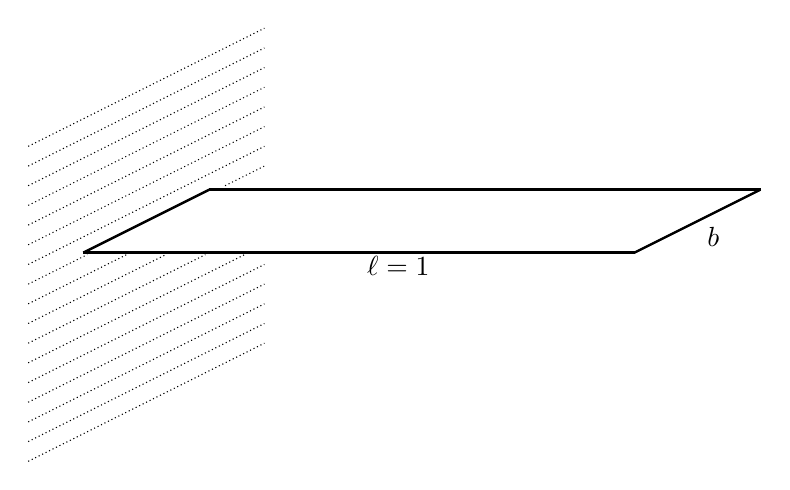
\begin{tikzpicture}
					\draw[line width = 0.3mm] (-0.8,-0.1) -- (6.2,-0.1);
					\draw[line width = 0.3mm] (0.8,0.7) -- (7.8,0.7);
					\draw[line width = 0.3mm] (-0.8,-0.1) -- (0.8,0.7);
					\draw[line width = 0.3mm] (6.2,-0.1) -- (7.8,0.7);
					
					
					
					\draw[scale=0.5, domain=-3:3, smooth, variable=\x,densely dotted] plot ({\x}, {0.5*\x+4});
					\draw[scale=0.5, domain=-3:3, smooth, variable=\x,densely dotted] plot ({\x}, {0.5*\x+3.5});
					\draw[scale=0.5, domain=-3:3, smooth, variable=\x,densely dotted] plot ({\x}, {0.5*\x+3});
					\draw[scale=0.5, domain=-3:3, smooth, variable=\x,densely dotted] plot ({\x}, {0.5*\x+2.5});
					\draw[scale=0.5, domain=-3:3, smooth, variable=\x,densely dotted] plot ({\x}, {0.5*\x+2});
					\draw[scale=0.5, domain=-3:3, smooth, variable=\x,densely dotted] plot ({\x}, {0.5*\x+1.5});
					\draw[scale=0.5, domain=-3:3, smooth, variable=\x,densely dotted] plot ({\x}, {0.5*\x+1});
					
					\draw[scale=0.5, domain=-3:-1.5, smooth, variable=\x,densely dotted] plot ({\x}, {0.5*\x+0.5});
					\draw[scale=0.5, domain=2:3, smooth, variable=\x,densely dotted] plot ({\x}, {0.5*\x+0.5});
					
					\draw[scale=0.5, domain=-3:-0.5, smooth, variable=\x,densely dotted] plot ({\x}, {0.5*\x});
					\draw[scale=0.5, domain=-3:0.5, smooth, variable=\x,densely dotted] plot ({\x}, {0.5*\x-0.5});
					\draw[scale=0.5, domain=-3:1.5, smooth, variable=\x,densely dotted] plot ({\x}, {0.5*\x-1});
					\draw[scale=0.5, domain=-3:2.5, smooth, variable=\x,densely dotted] plot ({\x}, {0.5*\x-1.5});
					\draw[scale=0.5, domain=-3:3, smooth, variable=\x,densely dotted] plot ({\x}, {0.5*\x-2});
					\draw[scale=0.5, domain=-3:3, smooth, variable=\x,densely dotted] plot ({\x}, {0.5*\x-2.5});
					\draw[scale=0.5, domain=-3:3, smooth, variable=\x,densely dotted] plot ({\x}, {0.5*\x-3});
					\draw[scale=0.5, domain=-3:3, smooth, variable=\x,densely dotted] plot ({\x}, {0.5*\x-3.5});
					\draw[scale=0.5, domain=-3:3, smooth, variable=\x,densely dotted] plot ({\x}, {0.5*\x-4});
					
					\node at (7.2,0.1) {$b$};
					\node at (3.2,-0.27) {$\ell = 1$};
										
					
					\draw[line width = 0.2mm] (0.8,0.7) -- (7.8,0.7);
					\draw[line width = 0.2mm] (-0.8,-0.1) -- (0.8,0.7);
					\draw[line width = 0.2mm] (6.2,-0.1) -- (7.8,0.7);
				\end{tikzpicture}
				\subcaption{Reissner-Mindlin cantilever plate}
			\end{minipage}
			\begin{minipage}[b]{0.8\linewidth}
				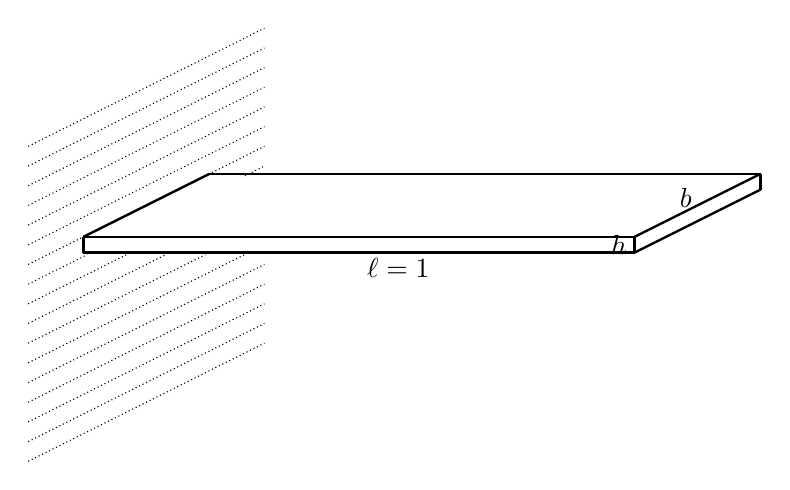
\begin{tikzpicture}
					\draw[line width = 0.3mm] (-0.8,0.1) -- (6.2,0.1);
					\draw[line width = 0.3mm] (-0.8,-0.1) -- (6.2,-0.1);
					\draw[line width = 0.3mm] (6.2,-0.1) -- (6.2,0.1);
					\draw[line width = 0.3mm] (-0.8,-0.1) -- (-0.8,0.1);
					
					\draw[line width = 0.3mm] (0.8,0.9) -- (7.8,0.9);
					\draw[line width = 0.3mm] (7.8,0.7) -- (7.8,0.9);
					
					\draw[line width = 0.3mm] (-0.8,0.1) -- (0.8,0.9);
					\draw[line width = 0.3mm] (6.2,0.1) -- (7.8,0.9);
					\draw[line width = 0.3mm] (6.2,-0.1) -- (7.8,0.7);
					
					
					
					\draw[scale=0.5, domain=-3:3, smooth, variable=\x,densely dotted] plot ({\x}, {0.5*\x+4});
					\draw[scale=0.5, domain=-3:3, smooth, variable=\x,densely dotted] plot ({\x}, {0.5*\x+3.5});
					\draw[scale=0.5, domain=-3:3, smooth, variable=\x,densely dotted] plot ({\x}, {0.5*\x+3});
					\draw[scale=0.5, domain=-3:3, smooth, variable=\x,densely dotted] plot ({\x}, {0.5*\x+2.5});
					\draw[scale=0.5, domain=-3:3, smooth, variable=\x,densely dotted] plot ({\x}, {0.5*\x+2});
					\draw[scale=0.5, domain=-3:3, smooth, variable=\x,densely dotted] plot ({\x}, {0.5*\x+1.5});
					\draw[scale=0.5, domain=-3:3, smooth, variable=\x,densely dotted] plot ({\x}, {0.5*\x+1});
					
					\draw[scale=0.5, domain=-3:-1.5, smooth, variable=\x,densely dotted] plot ({\x}, {0.5*\x+0.5});
					\draw[scale=0.5, domain=2.5:3, smooth, variable=\x,densely dotted] plot ({\x}, {0.5*\x+0.5});
					
					\draw[scale=0.5, domain=-3:-0.5, smooth, variable=\x,densely dotted] plot ({\x}, {0.5*\x});
					\draw[scale=0.5, domain=-3:0.5, smooth, variable=\x,densely dotted] plot ({\x}, {0.5*\x-0.5});
					\draw[scale=0.5, domain=-3:1.5, smooth, variable=\x,densely dotted] plot ({\x}, {0.5*\x-1});
					\draw[scale=0.5, domain=-3:2.5, smooth, variable=\x,densely dotted] plot ({\x}, {0.5*\x-1.5});
					\draw[scale=0.5, domain=-3:3, smooth, variable=\x,densely dotted] plot ({\x}, {0.5*\x-2});
					\draw[scale=0.5, domain=-3:3, smooth, variable=\x,densely dotted] plot ({\x}, {0.5*\x-2.5});
					\draw[scale=0.5, domain=-3:3, smooth, variable=\x,densely dotted] plot ({\x}, {0.5*\x-3});
					\draw[scale=0.5, domain=-3:3, smooth, variable=\x,densely dotted] plot ({\x}, {0.5*\x-3.5});
					\draw[scale=0.5, domain=-3:3, smooth, variable=\x,densely dotted] plot ({\x}, {0.5*\x-4});
					
					\node at (6.85,0.6) {$b$};
					\node at (6,0) {$h$};
					\node at (3.2,-0.3) {$\ell = 1$};
					
					% \draw[line width = 0.1mm,->] (9,1) -- (10,1.6);
					% \draw[line width = 0.1mm,->] (9,1) -- (10.4,1);
					% \draw[line width = 0.1mm,->] (9,1) -- (9,-0.1);
					% \node at (9.2,1.4) {$e_3$};
					% \node at (9.7,0.8) {$e_1$};
					% \node at (8.8,0.4) {$e_2$};
				\end{tikzpicture}
				\subcaption{Three-dimensional cantilever plate}
				
			\end{minipage}
		}
	}
\end{figure}
\FloatBarrier

\subsection{Calculating the eigenvalues}
The eigenvalues for both models are calculated using the Finite Element Method. For the plate model, the Finite Element Method is derived in \ref{sec:FEM:Plate} and for the three-dimensional model, the Finite Element Method is derived in \ref{sec:FEM:3D}. The eigenvalue problem for both models have the same form, but the matrices are different

\subsubsection{Problem 3D-1E and P-1E}
Find a vector function $u$ and a number $\lambda$ such that
\begin{eqnarray}
	K{u} & = & M\lambda{u}, 
\end{eqnarray} where $K$ and $M$ are the standard Finite Element Method matrices defined in section \ref{3d_fem_g} for Problem 3D-1E and section \ref{plate_fem_g} for Problem P-1E.

\subsubsection{Accuracy of the eigenvalues}
Figure \ref{fig:conv_3d_eig} show the rate of convergence of the first 20 eigenvalues of Problem 3D-1E. 

\begin{figure}[H]
    \centering
    \begin{adjustbox}{center}
        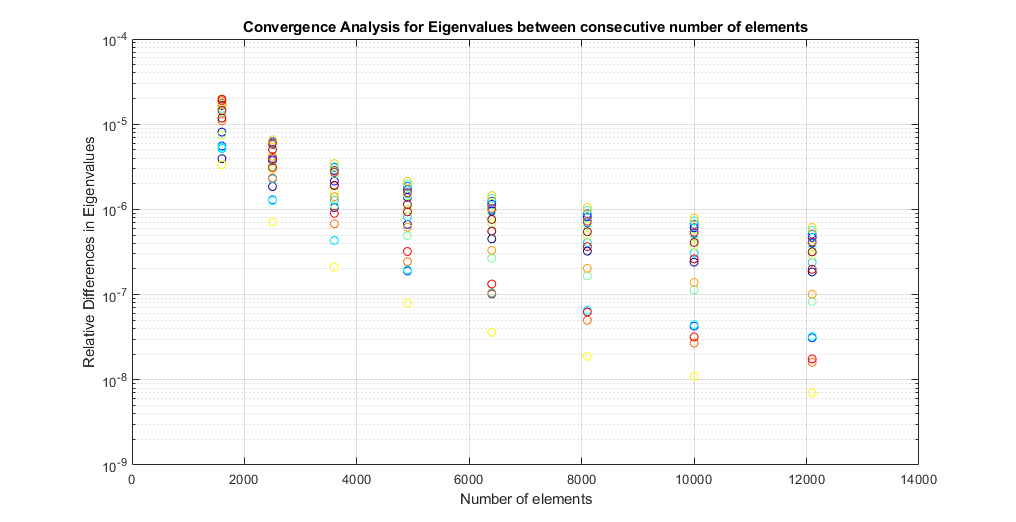
\includegraphics[scale=0.7]{Plate accuracy_no_legend.png}
    \end{adjustbox}
    \caption{Rate of convergence of the first 20 eigenvalues.}
    \label{fig:conv_3d_eig}
\end{figure}

The number of elements can be chosen so that at least the first 20 eigenvalues are accurate to 5 significant digits.

\subsection{Comparing the mode shapes}
Similar to the previous sections (section \ref{sec:validity-of-a-cantilever-timoshenko-beam} and section \ref{sec:validity-of-a-2d-beam}), the mode shapes of the two models are compared, to be able to match up the eigenvalues.

\subsubsection{Mode shapes relating to plate type eigenvalues}
Figure \ref{fig:plate_mode_shapes} shows examples of mode shapes relating to plate-type eigenvalues. The plate models has many different shapes.

\FloatBarrier
\begin{figure}[h!]
	\scalebox{.8}{
		\makebox[\textwidth][c]{
			\centering
			\begin{minipage}[b]{0.8\linewidth}
				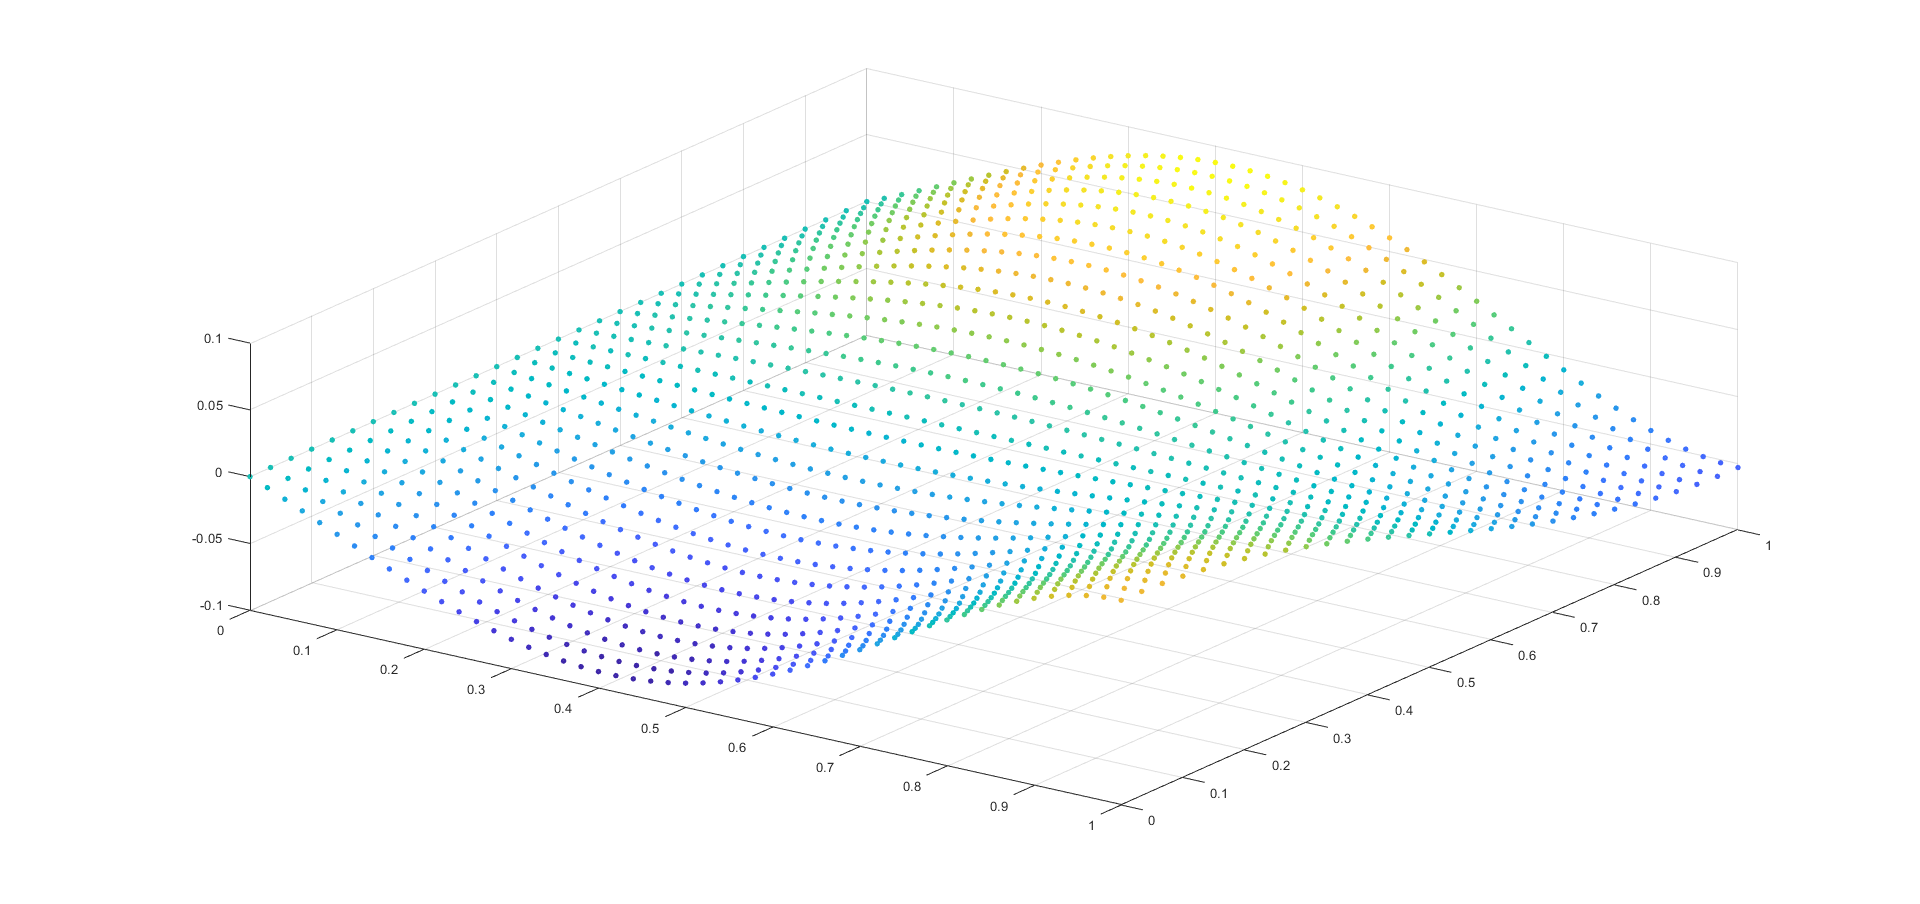
\includegraphics[width=1\linewidth]{Plate2.png}
				\subcaption{Plate - $\lambda_5 = 0.643$}
				\label{fig:minipage2}
			\end{minipage}
			\begin{minipage}[b]{0.8\linewidth}
				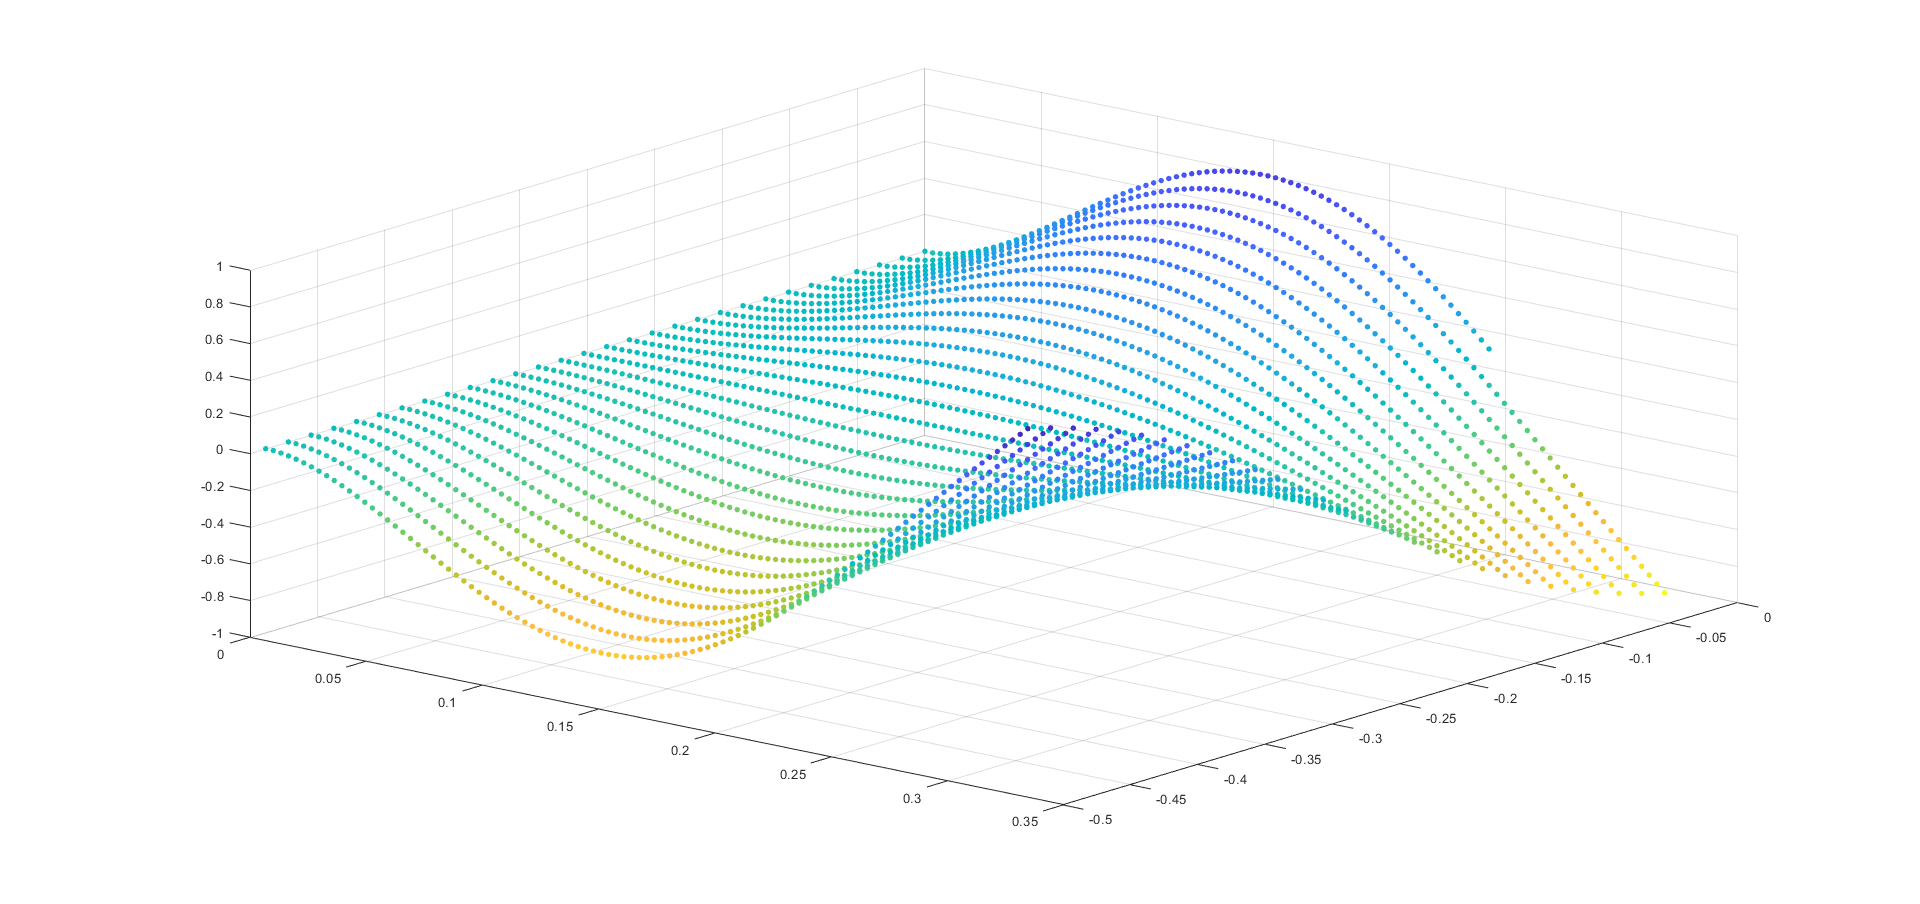
\includegraphics[width=1\linewidth]{3D2.png}
				\subcaption{3D Model - $\lambda_5 = 0.645$}
				\label{fig:minipage1}
			\end{minipage}
	}}
	\scalebox{.8}{
		\makebox[\textwidth][c]{
			\centering
			\begin{minipage}{.8\textwidth}
				\centering
				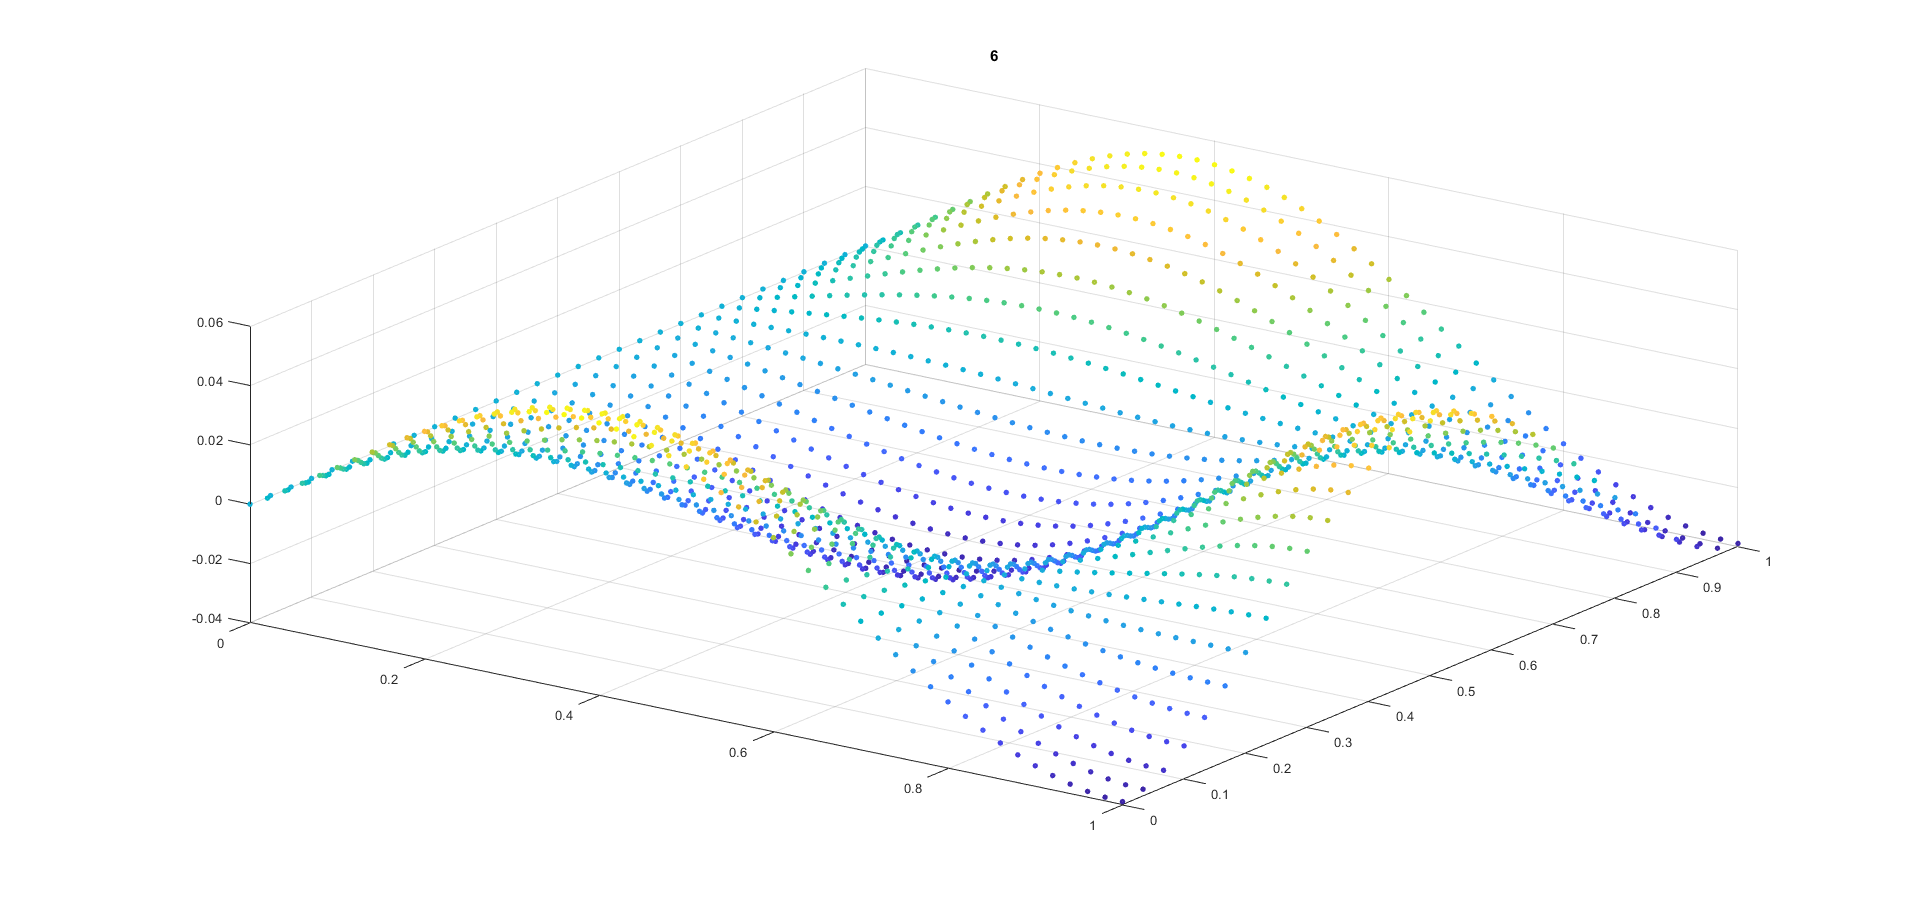
\includegraphics[width=1\linewidth]{Plate1.png}
				\subcaption{Plate - $\lambda_6 = 1.92$}
				\label{fig:minipage1}
			\end{minipage}
			\begin{minipage}{.8\textwidth}
				\centering
				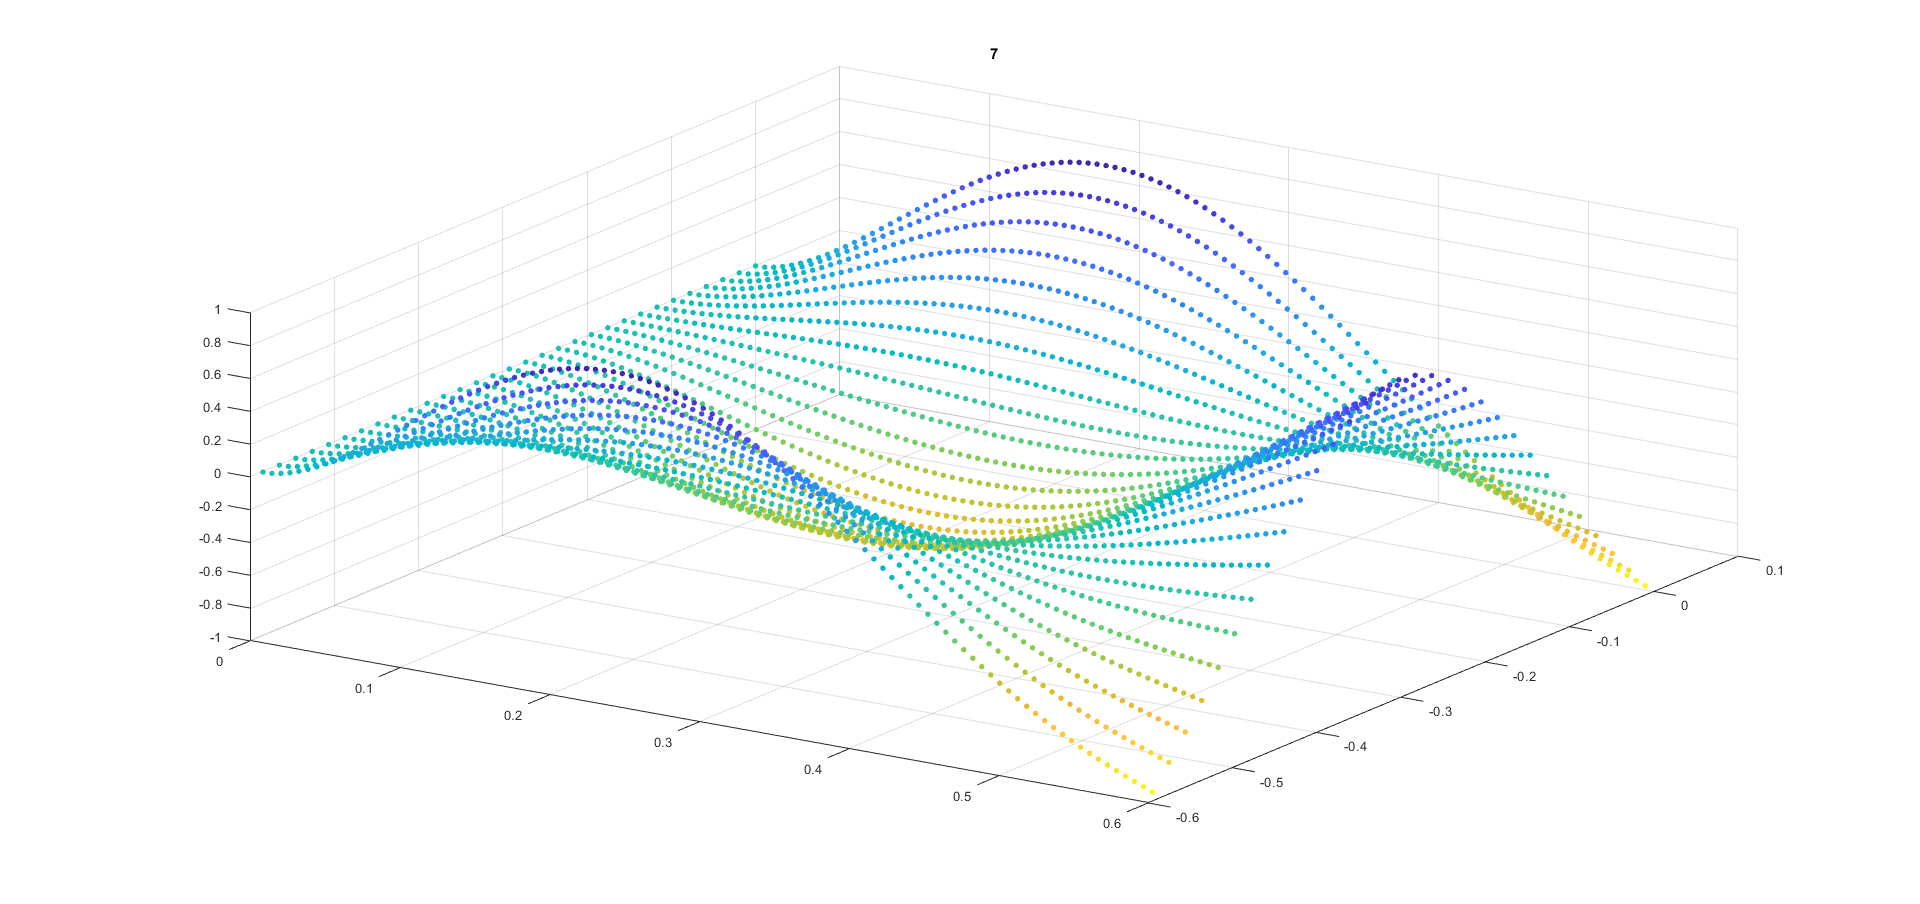
\includegraphics[width=1\linewidth]{3D1.png}
				\subcaption{3D Model - $\lambda_7 = 1.92$}
				\label{fig:minipage2}
			\end{minipage}
	}}
	\scalebox{.8}{
		\makebox[\textwidth][c]{
			\centering
			\begin{minipage}[b]{0.8\linewidth}
				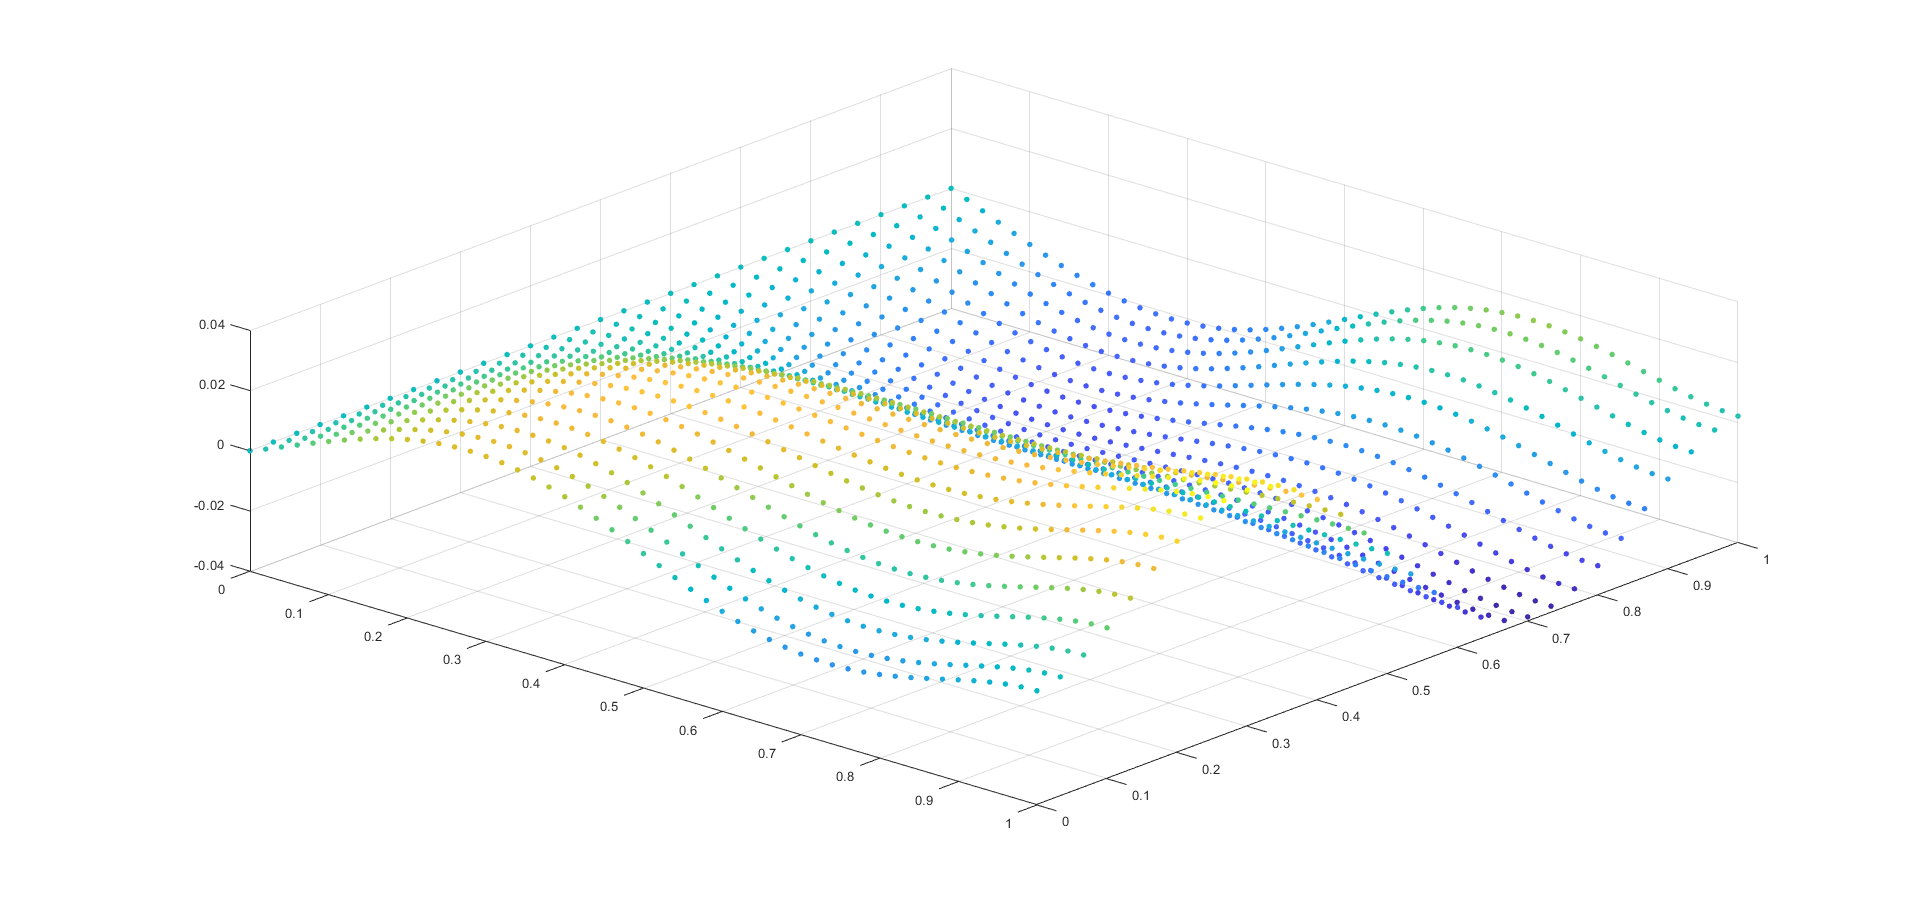
\includegraphics[width=1\linewidth]{Plate3.png}
				\subcaption{Plate - $\lambda_8 = 2.74$}
				\label{fig:minipage1}
			\end{minipage}
			\quad
			\begin{minipage}[b]{0.8\linewidth}
				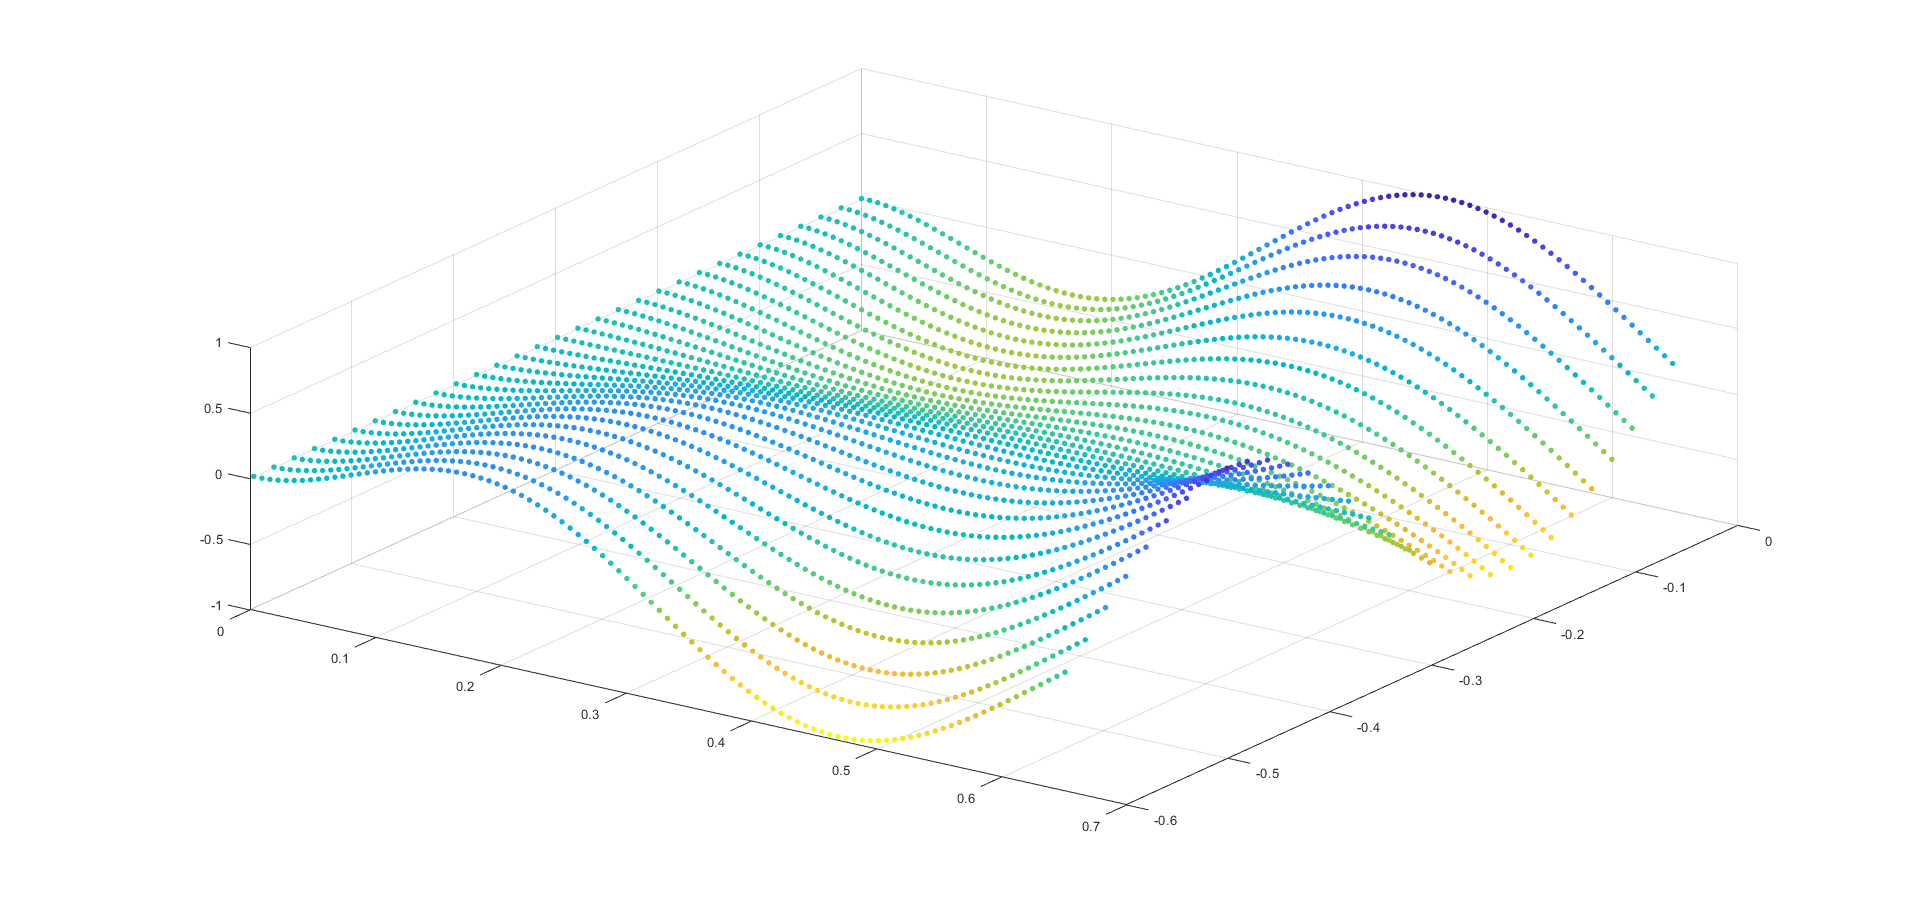
\includegraphics[width=1\linewidth]{3D3.png}
				\subcaption{3D Model - $\lambda_8 = 2.74$}
				\label{fig:minipage2}
			\end{minipage}
	}}
	\scalebox{.8}{
		\makebox[\textwidth][c]{
			\centering
			\begin{minipage}[b]{0.8\linewidth}
				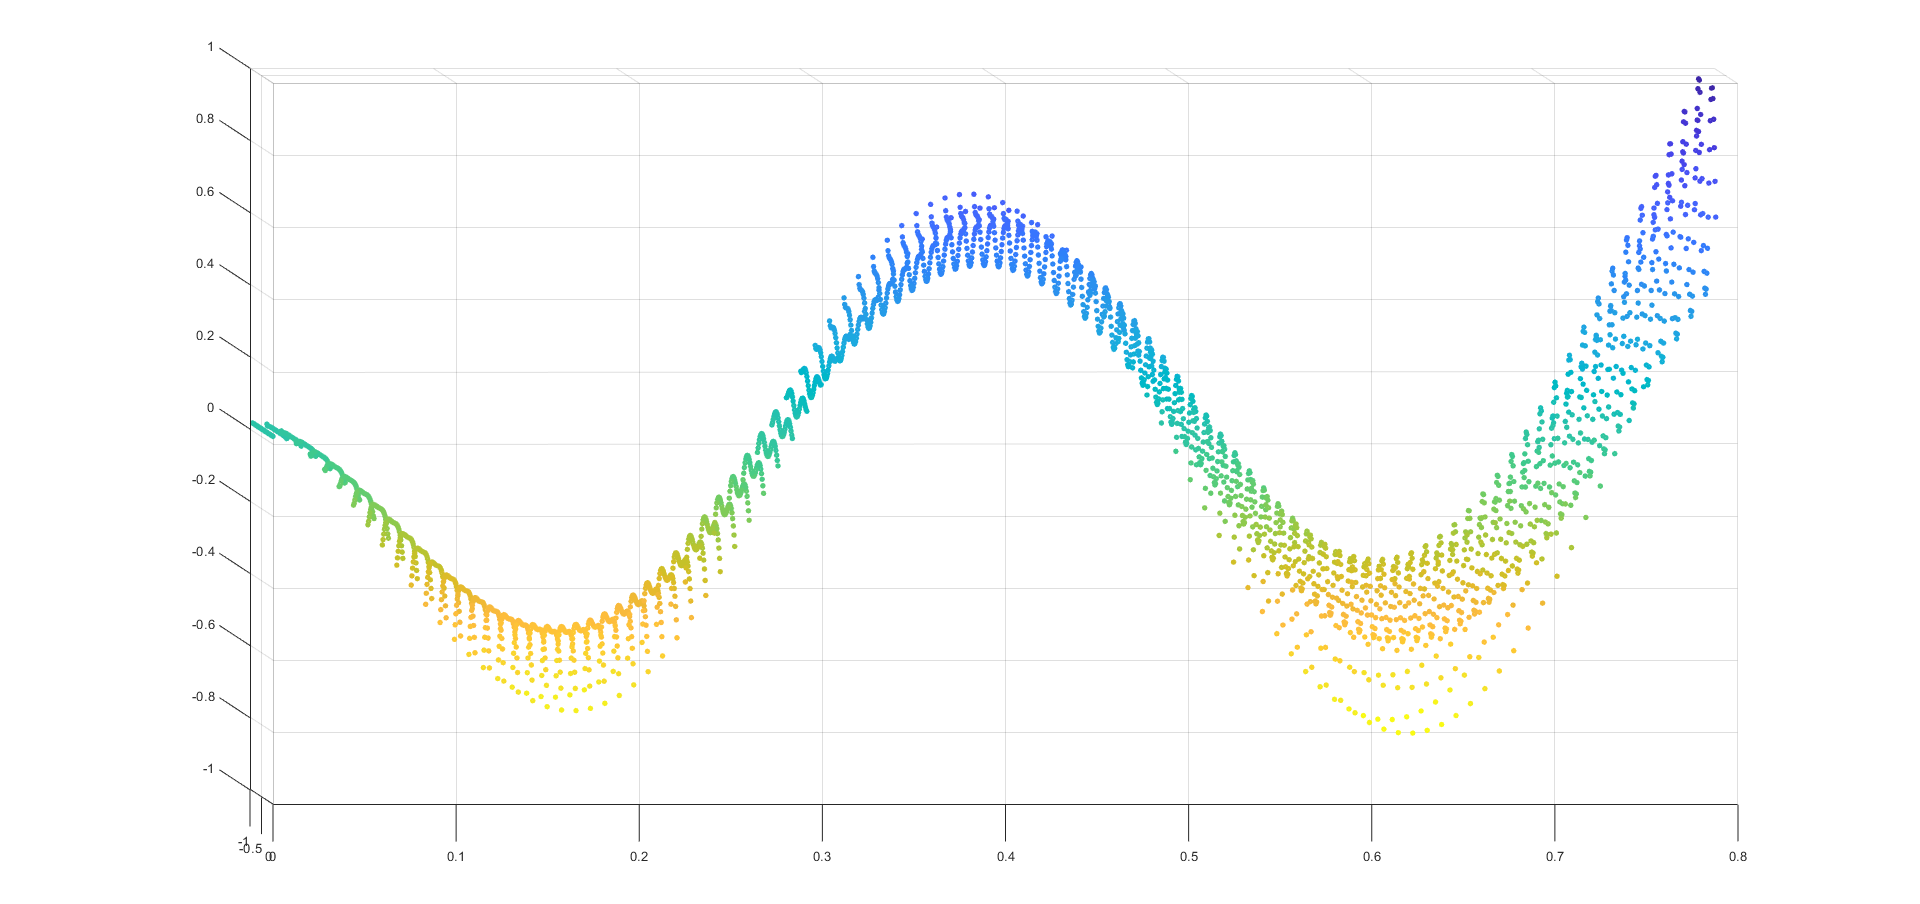
\includegraphics[width=1\linewidth]{Plate4.png}
				\subcaption{Plate - $\lambda_{12} = 8.96$ (Side view)}
				\label{fig:minipage2}
			\end{minipage}
			\quad
			\begin{minipage}[b]{0.8\linewidth}
				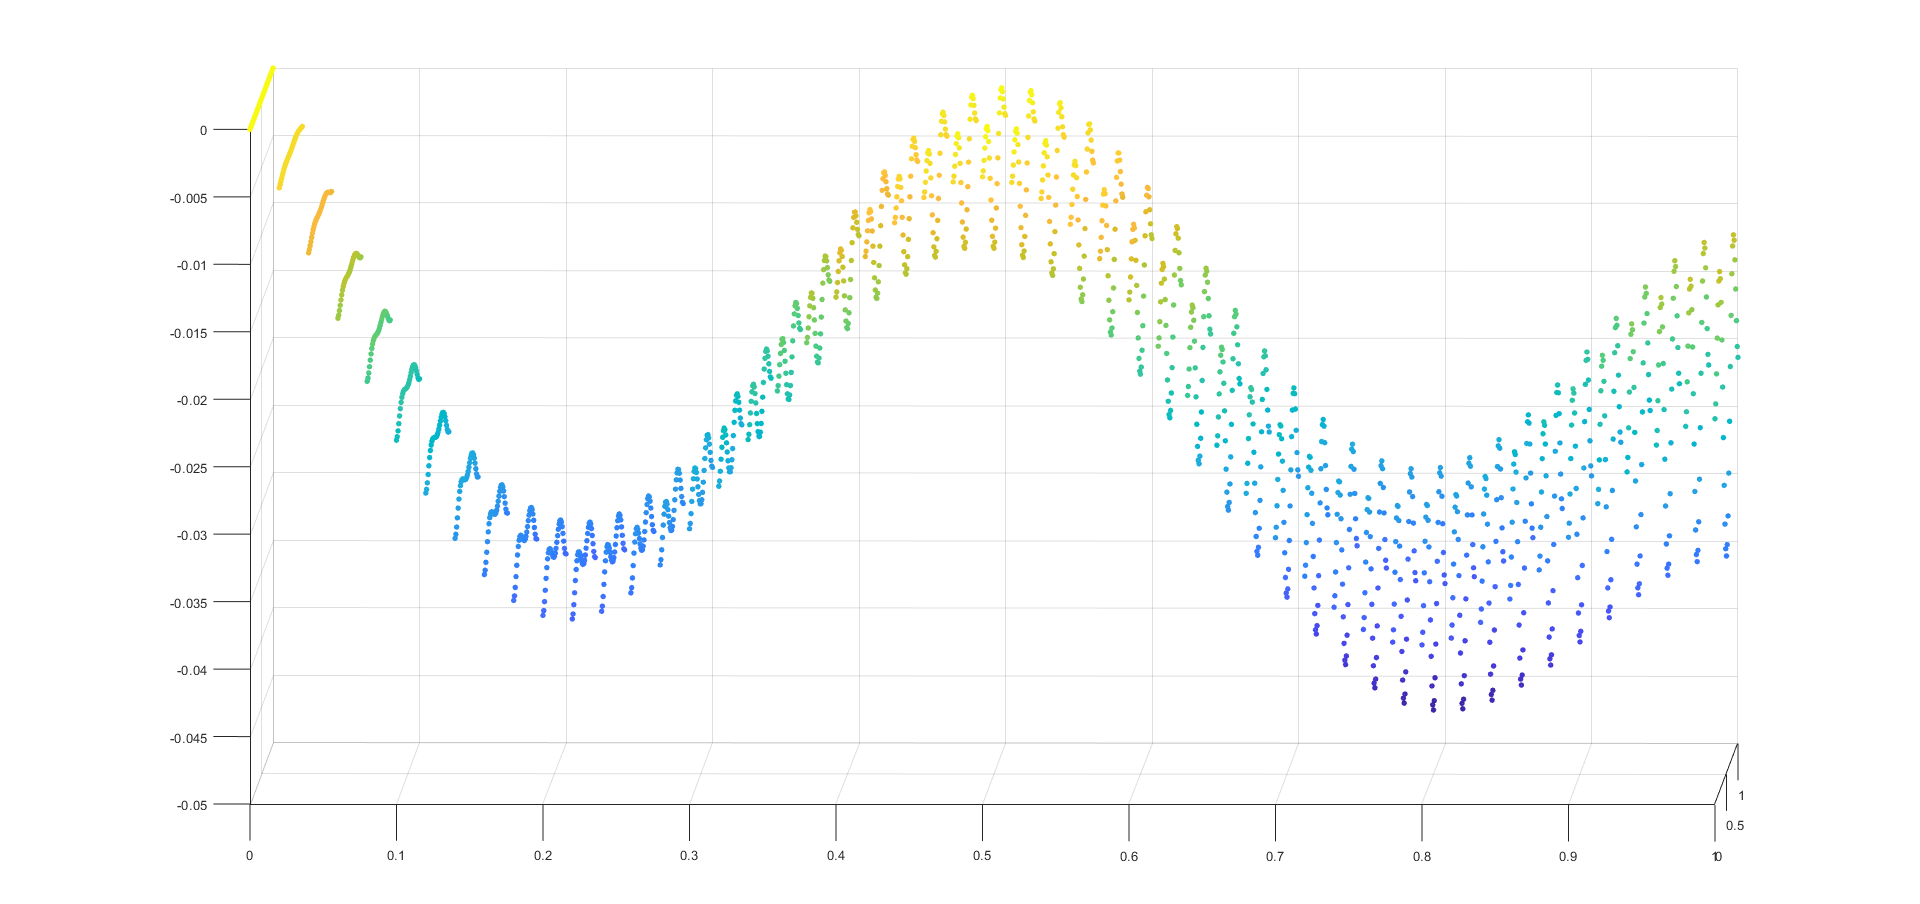
\includegraphics[width=1\linewidth]{3D4.png}
				\subcaption{3D Model - $\lambda_{14} = 9.01$ (Side view)}
				\label{fig:minipage2}
			\end{minipage}
			\caption{Comparison of mode shapes relating to plate-type models. $b = 1/20$, $d = 1$.}
	}}
\end{figure}\label{fig:plate_mode_shapes}
\FloatBarrier

\subsubsection{Mode shapes relating to non-plate type eigenvalues}
Figure \ref{fig:non_plate_mode_shapes} shows examples of mode shapes not relating to plate-type eigenvalues.

\begin{figure}[h!]
	\scalebox{.8}{
		\makebox[\textwidth][c]{
			\centering
			\begin{minipage}{.8\textwidth}
				\centering
				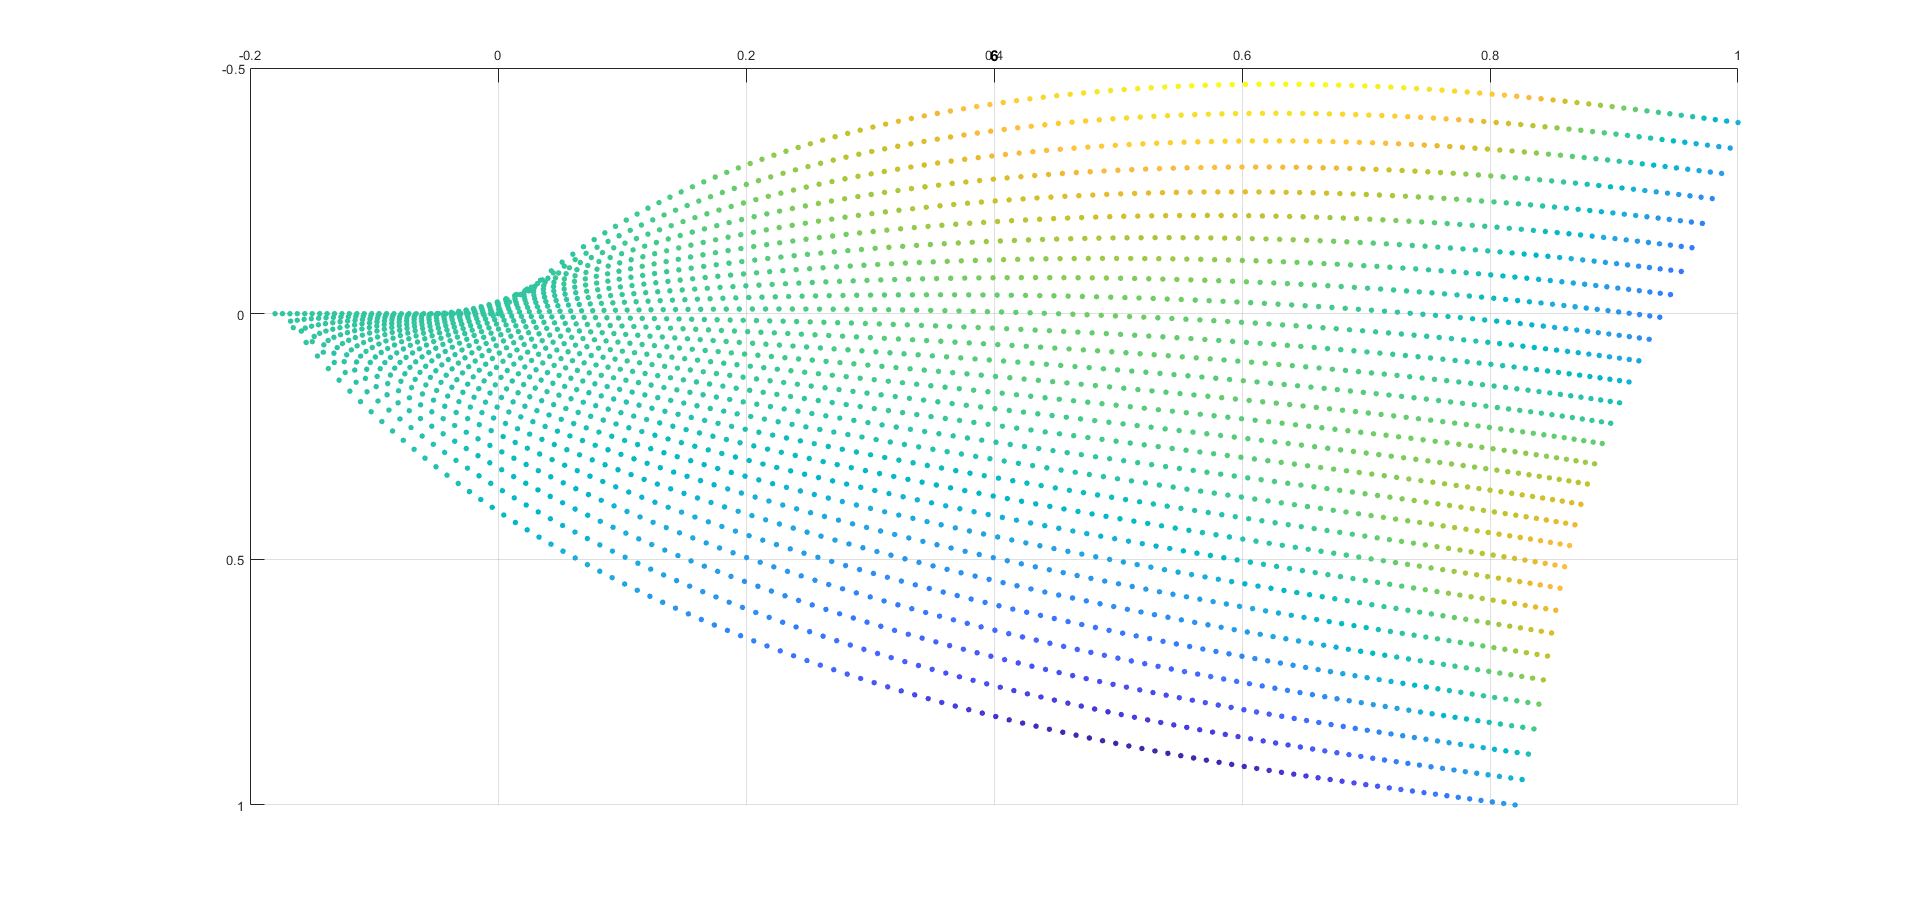
\includegraphics[width=1\linewidth]{3Dnp1.png}
				\subcaption{3D Model - $\lambda_{6} = 1.35$ (Top view)}
				\label{fig:minipage1}
			\end{minipage}
			\begin{minipage}{.8\textwidth}
				\centering
				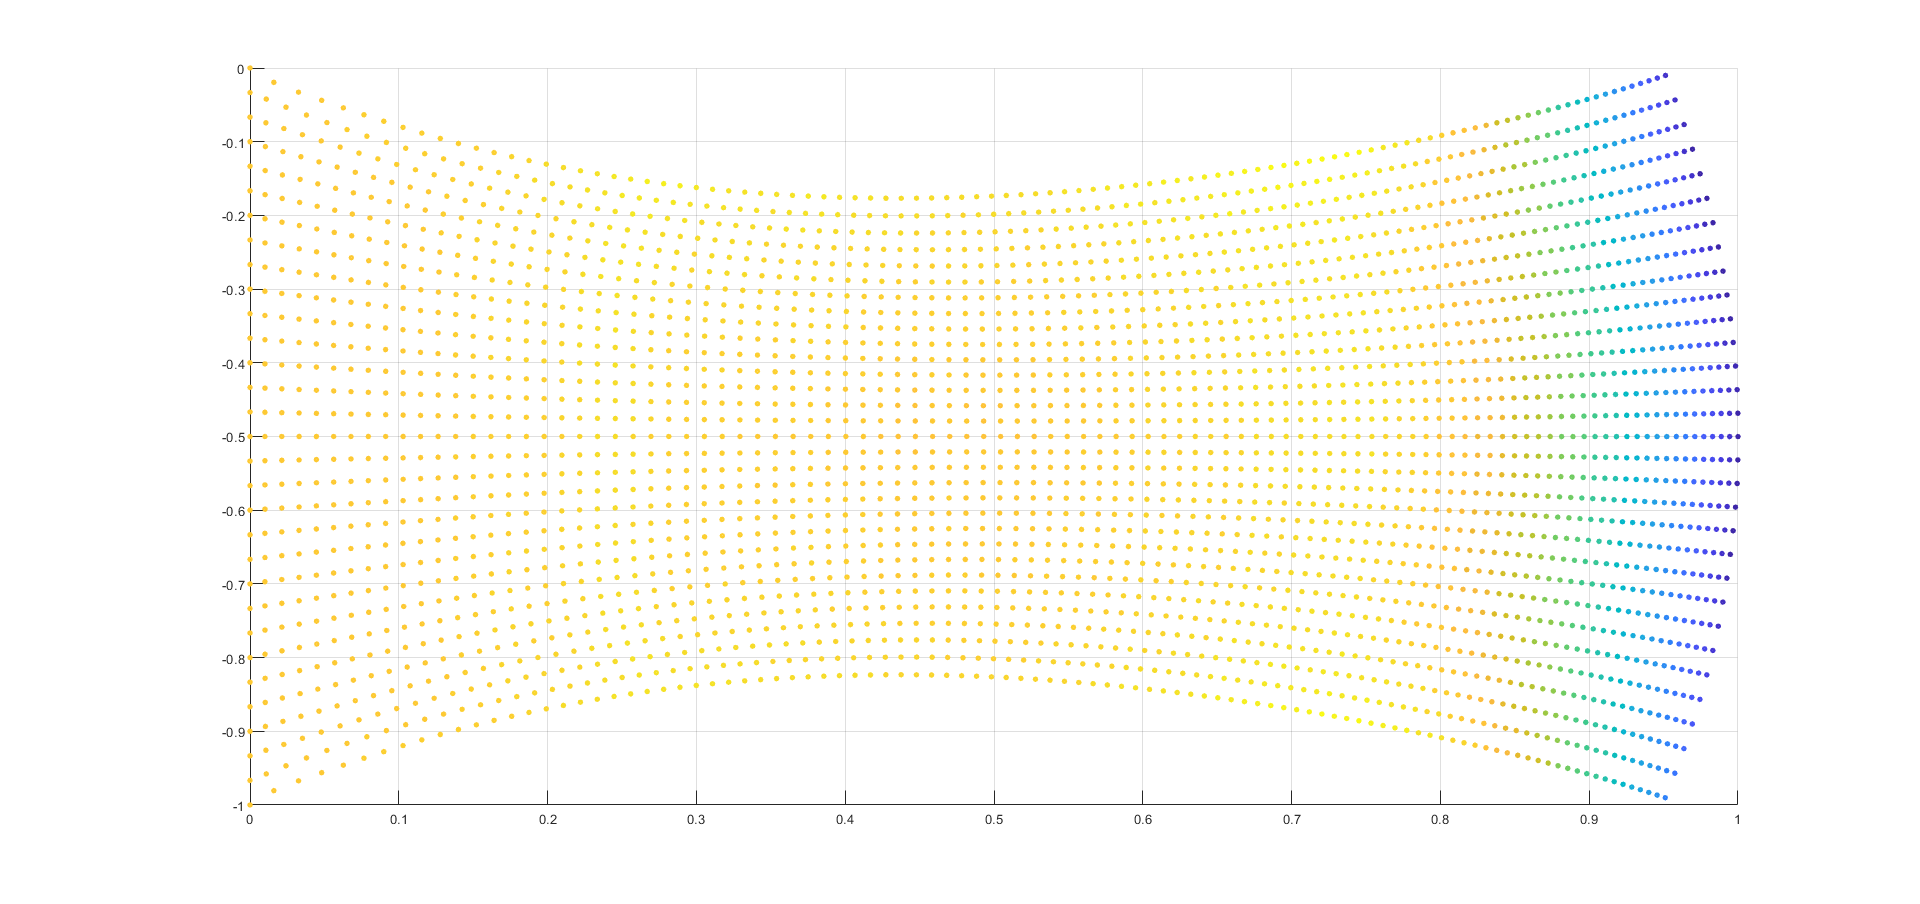
\includegraphics[width=1\linewidth]{3Dnp2.png}
				\subcaption{3D Model - $\lambda_{13} = 7.80$ (Top view)}
				\label{fig:minipage2}
			\end{minipage}
	}}
	\caption{Comparison of mode shapes not relating to plate-type models. $b = 1/20$, $d = 1$.}
\end{figure} \label{fig:non_plate_mode_shapes}


\subsection{Comparing the eigenvalues}
For a realistic comparison of the models, the parameters need to be chosen carefully. Both of the models have a width $h$ and a height $b$ parameter.

Three main cases are considered. These cases are $b = 0.25$ for a narrow plate, $b = 1$ for a plate with equal lenght and width and $b = 1.75$ for a wide plate. For each of the cases, the thickness of the plate is varied.

\textbf{Remark:} Note that the aim of the results is only to investigate the validity of the cantilever Reissner-Mindlin plate model, and not to investigate weather or not a plate model is more suited over beam model when applied to a body that has a larger width than height. 

\FloatBarrier
\begin{table}[htbp]
	\scalebox{.8}{
	\makebox[\textwidth]{
		\caption{Comparison of eigenvalues with $b = 0.25$, with decreasing values of $h$.}
		\begin{tabular}{|cccc||cccc||cccc||cccc|}
			\hline
			\multicolumn{16}{|c|}{Comparison of Eigenvalues, $b = 0.25$} \\
			\hline\hline
			\multicolumn{4}{|c||}{$h = 1/5$}       & \multicolumn{4}{c||}{$h =1/10$}      & \multicolumn{4}{c||}{$h = 1/20$}      & \multicolumn{4}{c|}{$h = 1/30$} \\
			\hline
			{i} & {3D} & {j} & {Plate} & {i} & {3D} & {j} & {Plate} & {i} & {3D} & {j} & {Plate} & {i} & {3D} & {j} & {Plate} \\
			\hline
			1     & 0.12348 & 1     & {0.12249} & 1     & 0.032327 & 1     & 0.032184 & 1     & 0.008207 & 1     & 0.008186 & 1     & 0.003663 & 1     & 0.003656 \\
			2     & 0.18638 &       & -     & 2     & 0.18531 &       & {-} & 2     & 0.18476 &       & {-} & 2     & 0.14204 & 2     & 0.14173 \\
			3     & 2.4151 & 2     & {2.3954} & 3     & 1.161 & 2     & 1.1537 & 3     & 0.31436 & 2     & 0.31341 & 3     & 0.18456 &       & {-} \\
			4     & 3.5856 & 3     & {3.5368} & 4     & 1.3155 & 3     & 1.31  & 4     & 0.44696 & 3     & 0.44582 & 4     & 0.21514 & 3     & 0.21454 \\
			5     & 4.785 &       & -     & 5     & 4.7697 &       & {-} & 5     & 2.3862 & 4     & 2.3767 & 5     & 1.1001 & 4     & 1.0971 \\
			6     & 7.7889 &       & -     & 6     & 7.7674 & 4     & 7.9816 & 6     & 4.1984 & 5     & 4.1857 & 6     & 2.0374 & 5     & 2.0313 \\
			7     & 20.37 & 4     & {19.969} & 7     & 8.056 &       & {-} & 7     & 4.7615 &       & {-} & 7     & 4.1509 & 6     & 4.1367 \\
			8     & 21.722 & 5     & {21.537} & 8     & 12.034 & 5     & 11.972 & 8     & 7.7543 &       & {-} & 8     & 4.7585 &       & {-} \\
			9     & 25.181 &       & -     & 9     & 25.147 &       & {-} & 9     & 8.7609 & 6     & 8.7132 & 9     & 6.2078 & 7     & 6.1864 \\
			10    & 56.321 & 6     & {54.887} & 10    & 26.608 & 6     & 26.266 & 10    & 12.598 & 7     & 12.548 & 10    & 7.7495 &       & {-} \\
			11    & 60.267 & 7     & {59.71} & 11    & 34.438 & 7     & 34.197 & 11    & 22.619 & 8     & 22.456 & 11    & 11.064 & 8     & 11.015 \\
			12    & 65.513 &       & -     & 12    & 61.829 & 8     & 60.801 & 12    & 25.128 &       & {-} & 12    & 13.734 & 9     & 13.678 \\
			13    & 69.031 &       & -     & 13    & 65.518 &       & {-} & 13    & 27.297 & 9     & 27.155 & 13    & 23.854 & 10    & 23.724 \\
			14    & 114.09 & 8     & {110.7} & 14    & 69.133 & 9     & 69.548 & 14    & 47.123 & 10    & 46.695 & 14    & 25.121 &       & {-} \\
			15    & 117.88 & 9     & {116.66} & 15    & 70.211 &       & {-} & 15    & 50.515 & 11    & 50.174 & 15    & 26.054 & 11    & 25.927 \\
			16    & 127.05 &       & -     & 16    & 116.78 & 10    & 114.43 & 16    & 65.523 &       & {-} & 16    & 36.259 & 12    & 36.15 \\
			17    & 184.46 & 10    & {185.78} & 17    & 121.43 & 11    & 119.94 & 17    & 69.089 &       & {-} & 17    & 41.973 & 13    & 41.807 \\
			18    & 191.91 & 11    & {191.47} & 18    & 127.23 &       & {-} & 18    & 71.563 & 12    & 71.166 & 18    & 44.95 & 14    & 44.685 \\
			19    & 193.03 &       & -     & 19    & 178.27 & 12    & 175.79 & 19    & 81.444 & 13    & 80.894 & 19    & 45.798 & 15    & 45.507 \\
			20    & 193.71 &       & -     & 20    & 186.06 & 13    & 187.28 & 20    & 84.785 & 14    & 84.064 & 20    & 54.838 & 16    & 54.573 \\
			\hline
			\multicolumn{2}{|c}{Max RE:} & \multicolumn{2}{c||}{2.9764\%} & \multicolumn{2}{c}{Max RE:} & \multicolumn{2}{c||}{2.7585\%} & \multicolumn{2}{c}{Max RE:} & \multicolumn{2}{c||}{0.90845\%} & \multicolumn{2}{c}{Max RE:} & \multicolumn{2}{c|}{0.63525\%} \\
			\hline
		\end{tabular}%
		\label{tab:Table_plate_1}%
	}}
\end{table}%
\FloatBarrier

\FloatBarrier
\begin{table}[htbp]
	\scalebox{.8}{
	\makebox[\textwidth]{
		\caption{Comparison of eigenvalues with $b = 1$, with decreasing values of $h$.}
		\begin{tabular}{|cccc||cccc||cccc||cccc|}
			\hline
			\multicolumn{16}{|c|}{Comparison of Eigenvalues, $b = 1$} \\
			\hline\hline
			\multicolumn{4}{|c||}{$h = 1/5$}       & \multicolumn{4}{c||}{$h =1/10$}      & \multicolumn{4}{c||}{$h = 1/20$}      & \multicolumn{4}{c|}{$h = 1/30$} \\
			\hline
			{i} & {3D} & {j} & {Plate} & {i} & {3D} & {j} & {Plate} & {i} & {3D} & {j} & {Plate} & {i} & {3D} & {j} & {Plate} \\
			\hline
			1     & 0.12869 & 1     & {0.12743} & 1     & 0.033784 & 1     & 0.033626 & 1     & 0.008565 & 1     & 0.008543 & 1     & 0.003817 & 1     & {0.00381} \\
			2     & 0.62189 & 2     & {0.61703} & 2     & 0.18635 & 2     & 0.18562 & 2     & 0.049829 & 2     & 0.04957 & 2     & 0.022511 & 2     & {0.022405} \\
			3     & 1.3638 &       & -     & 3     & 1.1603 & 3     & 1.153 & 3     & 0.31428 & 3     & 0.31315 & 3     & 0.14192 & 3     & {0.14156} \\
			4     & 3.5808 & 3     & {3.5289} & 4     & 1.3579 &       & {-} & 4     & 0.50842 & 4     & 0.50676 & 4     & 0.23035 & 4     & {0.22969} \\
			5     & 5.8165 & 4     & {5.7694} & 5     & 1.864 & 4     & 1.8577 & 5     & 0.64595 & 5     & 0.64297 & 5     & 0.29502 & 5     & {0.29394} \\
			6     & 6.6048 & 5     & {6.5216} & 6     & 2.2928 & 5     & 2.2792 & 6     & 1.3555 &       & {-} & 6     & 0.8928 & 6     & {0.88735} \\
			7     & 7.8455 &       & -     & 7     & 6.4973 & 6     & 6.4546 & 7     & 1.9293 & 6     & 1.9157 & 7     & 1.156 & 7     & {1.1527} \\
			8     & 9.8027 &       & -     & 8     & 7.8167 &       & {-} & 8     & 2.5089 & 7     & 2.4975 & 8     & 1.265 & 8     & {1.261} \\
			9     & 17.03 & 6     & {16.802} & 9     & 8.4533 & 7     & 8.3671 & 9     & 2.7486 & 8     & 2.7369 & 9     & 1.3543 &       & - \\
			10    & 21.225 & 7     & {20.743} & 10    & 9.3453 & 8     & 9.2873 & 10    & 3.3087 & 9     & 3.2903 & 10    & 1.5352 & 9     & {1.529} \\
			11    & 23.935 & 8     & {23.552} & 11    & 9.8009 &       & {-} & 11    & 5.5365 & 10    & 5.4914 & 11    & 2.598 & 10    & {2.5803} \\
			12    & 24.694 &       & -     & 12    & 10.925 & 9     & 10.827 & 12    & 5.9696 & 11    & 5.9246 & 12    & 2.8161 & 11    & {2.7997} \\
			13    & 27.187 & 9     & {26.69} & 13    & 17.599 & 10    & 17.447 & 13    & 7.8024 &       & {-} & 13    & 4.2654 & 12    & {4.2474} \\
			14    & 28.844 &       & -     & 14    & 18.596 & 11    & 18.407 & 14    & 9.0173 & 12    & 8.9573 & 14    & 4.6674 & 13    & {4.6415} \\
			15    & 32.373 &       & -     & 15    & 24.729 &       & {-} & 15    & 9.8006 & 13    & 9.838 & 15    & 4.9397 & 14    & {4.9143} \\
			16    & 41.288 & 10    & {40.519} & 16    & 27.4  & 12    & 27.021 & 16    & 9.9172 &       & {-} & 16    & 5.7243 & 15    & {5.6803} \\
			17    & 42.082 & 11    & {41.246} & 17    & 28.81 &       & {-} & 17    & 10.365 & 13    & 10.286 & 17    & 6.6585 & 16    & {6.6025} \\
			18    & 51.427 &       & -     & 18    & 30.737 & 13    & 30.413 & 18    & 11.934 & 14    & 11.817 & 18    & 7.2935 & 17    & {7.2474} \\
			19    & 56.963 & 12    & {56.1} & 19    & 30.83 & 14    & 30.413 & 19    & 13.915 & 15    & 13.767 & 19    & 7.7966 &       & - \\
			20    & 57.741 &       & -     & 20    & 32.414 &       &       & 20    & 15.109 & 16    & 14.974 & 20    & 9.7996 &       & - \\
			\hline
			\multicolumn{2}{|c}{Max RE:} & \multicolumn{2}{c||}{2.2695\%} & \multicolumn{2}{c}{Max RE:} & \multicolumn{2}{c||}{1.3816\%} & \multicolumn{2}{c}{Max RE:} & \multicolumn{2}{c||}{1.0657\%} & \multicolumn{2}{c}{Max RE:} & \multicolumn{2}{c|}{0.84102\%} \\
			\hline
		\end{tabular}%
		\label{tab:Table_plate_2}%
	}}
\end{table}%
\FloatBarrier


\FloatBarrier
\begin{table}[htbp]
	\scalebox{.8}{
	\makebox[\textwidth]{
		\caption{Comparison of eigenvalues with $b = 1.75$, with decreasing values of $h$.}
		\begin{tabular}{|cccc||cccc||cccc||cccc|}
			\hline
			\multicolumn{16}{|c|}{Comparison of Eigenvalues, $b = 1.75$} \\
			\hline\hline
			\multicolumn{4}{|c||}{$h = 1/5$}       & \multicolumn{4}{c||}{$h =1/10$}      & \multicolumn{4}{c||}{$h = 1/20$}      & \multicolumn{4}{c|}{$h = 1/30$} \\
			\hline
			{i} & {3D} & {j} & {Plate} & {i} & {3D} & {j} & {Plate} & {i} & {3D} & {j} & {Plate} & {i} & {3D} & {j} & {Plate} \\
			\hline
			1 & 0.13062 & 1 & 0.12939 & 1 & 0.034245 & 1 & 0.034079 & 1 & 0.0086697 & 1 & 0.0086456 & 1 & 0.0038626 & 1 & 0.0038541\\
			2 & 0.32016 & 2 & 0.31779 & 2 & 0.089872 & 2 & 0.089508 & 2 & 0.023395 & 2 & 0.023323 & 2 & 0.010507 & 2 & 0.010475\\
			3 & 1.2496 & 3 & 1.2422 & 3 & 0.36964 & 3 & 0.36841 & 3 & 0.098072 & 3 & 0.097745 & 3 & 0.044239 & 3 & 0.044074\\
			4 & 1.9808 &  & - & 4 & 1.2274 & 4 & 1.2188 & 4 & 0.33233 & 4 & 0.33118 & 4 & 0.15003 & 4 & 0.14964\\
			5 & 3.7675 & 4 & 3.7086 & 5 & 1.352 & 5 & 1.3465 & 5 & 0.36764 & 5 & 0.36652 & 5 & 0.16657 & 5 & 0.16605\\
			6 & 4.2021 & 5 & 4.1631 & 6 & 1.6994 & 6 & 1.6894 & 6 & 0.4647 & 6 & 0.4632 & 6 & 0.21059 & 6 & 0.21002\\
			7 & 5.2022 & 6 & 5.1381 & 7 & 1.9763 &  & - & 7 & 0.79935 & 7 & 0.79606 & 7 & 0.3656 & 7 & 0.36423\\
			8 & 7.6603 & 7 & 7.9399 & 8 & 2.8259 & 7 & 2.8076 & 8 & 1.2445 & 8 & 1.2411 & 8 & 0.56685 & 8 & 0.56529\\
			9 & 8.0445 &  & - & 9 & 4.4507 & 8 & 4.4294 & 9 & 1.5708 & 9 & 1.563 & 9 & 0.72384 & 9 & 0.72032\\
			10 & 9.0791 &  & - & 10 & 5.3923 & 9 & 5.3539 & 10 & 1.9739 &  & - & 10 & 1.1585 & 10 & 1.1545\\
			11 & 10.135 &  & - & 11 & 7.6371 &  & 0 & 11 & 2.5137 & 10 & 2.5015 & 11 & 1.2513 & 11 & 1.2466\\
			12 & 12.888 & 8 & 12.736 & 12 & 8.4707 & 10 & 8.3817 & 12 & 2.708 & 11 & 2.6947 & 12 & 1.4005 & 12 & 1.3927\\
			13 & 14.506 & 9 & 14.302 & 13 & 9.0612 & 11 & 8.9704 & 13 & 3.0153 & 12 & 2.9984 & 13 & 1.4449 & 13 & 1.4393\\
			14 & 14.892 &  & - & 14 & 9.0682 & & - & 14 & 3.137 & 13 & 3.1246 & 14 & 1.6806 & 14 & 1.6738\\
			15 & 19.395 &  & - & 15 & 10.018 & 12 & 9.9347 & 15 & 3.6118 & 14 & 3.5928 & 15 & 1.973 &  & -\\
			16 & 21.265 & 10 & 20.79 & 16 & 10.131 &  & - & 16 & 5.1287 & 15 & 5.0977 & 16 & 2.4081 & 15 & 2.3958\\
			17 & 22.512 & 11 & 22.038 & 17 & 10.683 & 13 & 10.605 & 17 & 5.6368 & 16 & 5.6009 & 17 & 2.6419 & 16 & 2.6253\\
			18 & 25.193 & 12 & 24.775 & 18 & 11.806 & 14 & 11.682 & 18 & 6.5069 & 17 & 6.4687 & 18 & 3.0386 & 17 & 3.0189\\
			19 & 27.783 & 13 & 27.322 & 19 & 14.893 &  & - & 19 & 7.6243 & 18 & 7.6617 & 19 & 3.6563 & 18 & 3.6342\\
			20 & 28.461 & 14 & 27.851 & 20 & 16.275 & 15 & 16.1 & 20 & 7.7152 &  & - & 20 & 4.3466 & 19 & 4.3267\\
			\hline
			\multicolumn{2}{|c}{Max RE:} & \multicolumn{2}{c||}{3.6499\%} & \multicolumn{2}{c}{Max RE:} & \multicolumn{2}{c||}{1.0878\%} & \multicolumn{2}{c}{Max RE:} & \multicolumn{2}{c||}{0.63674\%} & \multicolumn{2}{c}{Max RE:} & \multicolumn{2}{c|}{0.64798\%} \\
			\hline
		\end{tabular}
		\label{tab:Table_plate_3}
	}}
\end{table}
\FloatBarrier

Overall Tables \ref{tab:Table_plate_1}, \ref{tab:Table_plate_2} and \ref{tab:Table_plate_3} shows that the cantilever Reissner-Mindlin plate model compares very well to the three-dimensional plate. The maximum relative error is less than 3.65\% for all cases considered.

There is less of a dramatic change of the comparison when the width of the plate is changed as with the beam model in section \ref{sec:validity-of-a-2d-beam}. This could be because the Reissner-Mindlin plate model does consider both the width and the height of the plate, while it is only a two-dimensional model. The two-dimensional beam model only considered the height of the beam, and not the width.

Other cases not shown here have also been considered, and the results are similar to the ones shown here. They are therefore not included here, and only worth mentioning.

\end{document}